\chapter{Apprendimento democratizzato: Algoritmo e risultati}\label{ch:chapter4}
Riportiamo di seguito il DemLearn tramite uno pseudocodice.

\begin{algorithm}[H]
 \KwData{K, T, $\tau$}
 \For{t=0,...,T-1}{
 	\For{learning agent n=1,...,N}{
 	L'agente \textsl{n} usa il modello del gruppo superiore $w_{n,t}^{(1)}$ come modello iniziale. L'agente \textsl{n} aggiorna iterativamente il modello di apprendimento personalizzato $w_{(n,t+1)}^{(0)}$ come minimizzatore inesatto,  ovvero basato sul gradiente, del seguente problema: $min_{w\in W}L_n^{(0)}(w|D_n)+\frac{\mu}{2}||w-w_{(n,t)}^{(1)}||^2$ \hspace{1cm} (8) L'agente \textsl{n} invia il modello di apprendimento aggiornato al server.
 	}
 	\If{t mod $\tau$=0} {
 	Il server ricostruisce la struttura gerarchica mediante l'algoritmo di clustering.
 	}
 	Aggiornamento gerarchico: ogni gruppo i ad ogni livello k esegue un aggiornamento per il suo modello di apprendimento dal basso verso l'alto per aggiornare il contributo dei membri del gruppo. $w_{(i,t+1)}^{(k)}=\sum_{j\in S_{(i,k)}}\frac{N_{(g,j)}^{(k-1)}}{N_{(g,i)}^{(k)}}w_{(j,t+1)}^{(k-1)}$\hspace{1cm} (9) Dopo che il modello di livello superiore è stato aggiornato, i livelli inferiori iniziano ad aggiornarsi dall'alto verso il basso per il contributo del gruppo superiore come segue: $w_{(i,t+1)}^{(k)}=\alpha w_{(t+1)}^{(k+1)}+(1-\alpha )w_{(i,t+1)}^{(k)}$ \hspace{1cm} (10) I modelli di apprendimento aggiornati al livello 1 (vale a dire, $w_{(t+1)}^{(1)}$) vengono quindi trasmessi a tutti gli agenti per aggiornare i loro modelli locali seguendo l'equazione (10).}
\caption{Algoritmo democratizzato}
\end{algorithm}
In questo paragrafo, convalidiamo l'efficacia dell'algoritmo DemLearn con MNIST, Fashion-MNIST [21], Set di dati Federated Extended MNIST e CIFAR-10 rispettivamente per il riconoscimento di cifre scritte a mano, immagini di moda e per il riconoscimento di oggetti. Conduciamo gli esperimenti con 50 clienti, in cui ogni cliente ha numeri mediani di campioni di dati a 64, 70 e 785 con MNIST, set di dati Fashion MNIST e CIFAR-10, rispettivamente. Diversamente da questi tre set di dati, sperimentiamo anche il set di dati FE-MNIST che ha un numero maggiore di classi come 10 cifre, 25 minuscole e 25 maiuscole. Di conseguenza, selezioniamo 50 clienti da 3559 utenti che hanno almeno 50 campioni di dati nel set di dati FE-MNIST. Utilizzando questi set di dati, il 20\% dei campioni di dati su ciascun client viene utilizzato per valutare le prestazioni di test del modello. Dividiamo il set di dati totale in modo tale che ogni cliente disponga di una piccola quantità di dati da due etichette specifiche tra i dieci complessivi in entrambi i set di dati. In tal modo, replichiamo uno scenario di set di dati personali distorti, ovvero dati altamente sbilanciati e un numero limitato di campioni di addestramento possono essere raccolti presso gli agenti. I modelli di apprendimento sono costituiti da due livelli di convoluzione seguiti da due livelli di pooling e due livelli completamente connessi, mentre nel set di dati CIFAR-10 vengono utilizzati tre livelli di convoluzione. Impostiamo il periodo di aggiornamento $\tau=1$ e convalidiamo le prestazioni della proposta algoritmo con K = 4 livelli generalizzati. DemLearn, FedAvg e FedProx utilizzano il tasso di apprendimento comune $\eta$ = 0.05, epoca locale E = 2, dimensione batch B = 10.
Per FedProx, impostiamo il parametro $\tau$ = 0,5. Nel frattempo, pFedMe necessita di una messa a punto dettagliata per ottenere un'accuratezza competitiva per diversi set di dati.\\
Gli approcci FL esistenti come FedProx e FedAvg si concentrano maggiormente sulle prestazioni di apprendimento del modello globale piuttosto che sulle prestazioni di apprendimento dei clienti. Pertanto, per le prossime applicazioni personalizzate, implementiamo DemLearn e misuriamo le prestazioni di apprendimento di tutti i clienti e dei modelli di gruppo. In particolare, conduciamo valutazioni per la specializzazione (C-SPE) e la generalizzazione (C-GEN) dei modelli di apprendimento in media presso gli agenti che sono definiti solo come le prestazioni nei loro dati di test locali e i dati di test collettivi di tutti gli agenti nella regione. Di conseguenza, indichiamo Global come prestazione del modello globale; e GGEN e G-SPE sono rispettivamente le prestazioni medie di generalizzazione e specializzazione dei modelli di gruppo. Oltre alle prestazioni C-SPE standard per i modelli locali, le prestazioni C-GEN introdotte sono una metrica importante che mostra le capacità generalizzate dei modelli locali. Anche se i modelli locali distorti possono raggiungere valori C-SPE elevati fin dall'inizio, in particolare a causa dei loro piccoli set di dati locali, hanno ancora capacità generalizzate molto basse che possono aiutare a produrre buone previsioni in base ai frequenti cambiamenti degli utenti. Nel frattempo, i modelli globali e di gruppo hanno le capacità generalizzate più elevate, ma capacità specializzate inferiori durante la distribuzione ai client.\\\\
Nelle figure seguenti sono stati condotti alcuni confronti delle prestazioni con i seguenti metodi, DemLearn con i tre metodi FL, FedAvg, FedProx e pFedMe come linee di base su quattro set di dati di riferimento, MNIST, Fashion MNIST, FE- MNIST e CIFAR-10. Le valutazioni sperimentali mostrano che l'approccio proposto supera le linee di base in termini di velocità di convergenza, in particolare per ottenere migliori prestazioni di generalizzazione del client. Osserviamo che il modello locale richiede solo 40 round per raggiungere il livello di prestazioni C-GEN dell'80\% utilizzando l'algoritmo proposto, mentre gli algoritmi FL esistenti come FedProx, FedAvg e pFedMe impiegano più di 80 round globali per raggiungere un livello quasi competitivo livello di prestazioni come il nostro. Inoltre, dopo 100 round, Dem Learn ottiene prestazioni di generalizzazione del cliente medie migliori (ad esempio, 88,77\%) tra i modelli di client e prestazioni C-SPE  comparabili a partire da FedAvg e pFedMe.\\
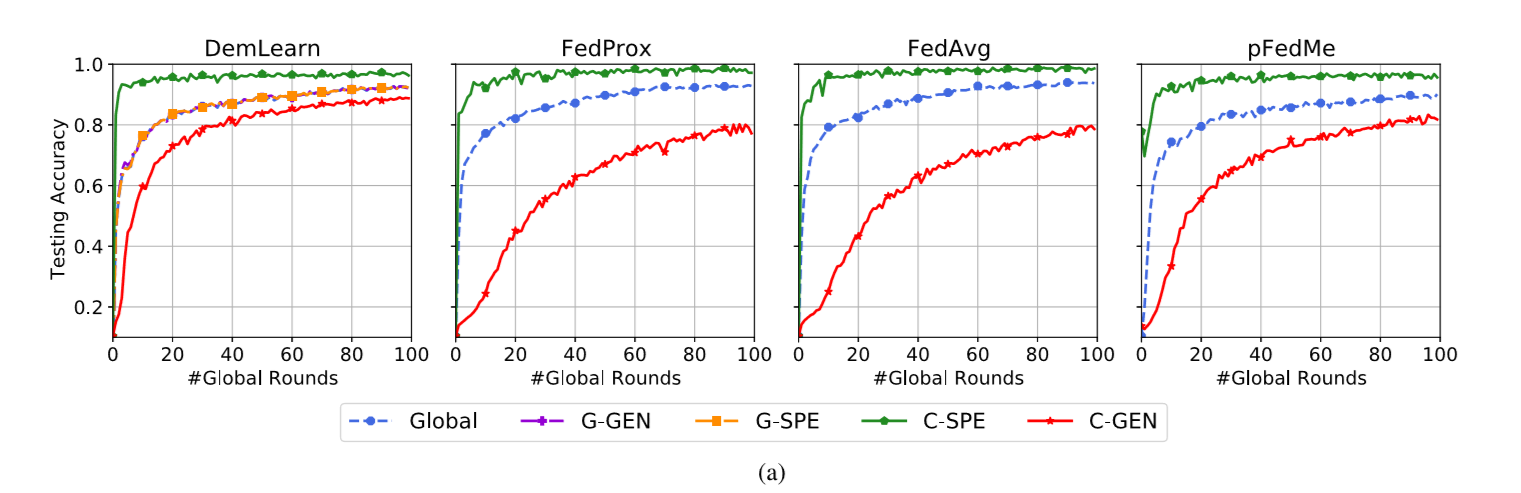
\includegraphics[scale=0.4]{DemLearnMNIST}\\
Notiamo che DemLearn ha prestazioni nettamente superiori con il set di dati MNIST\\\\
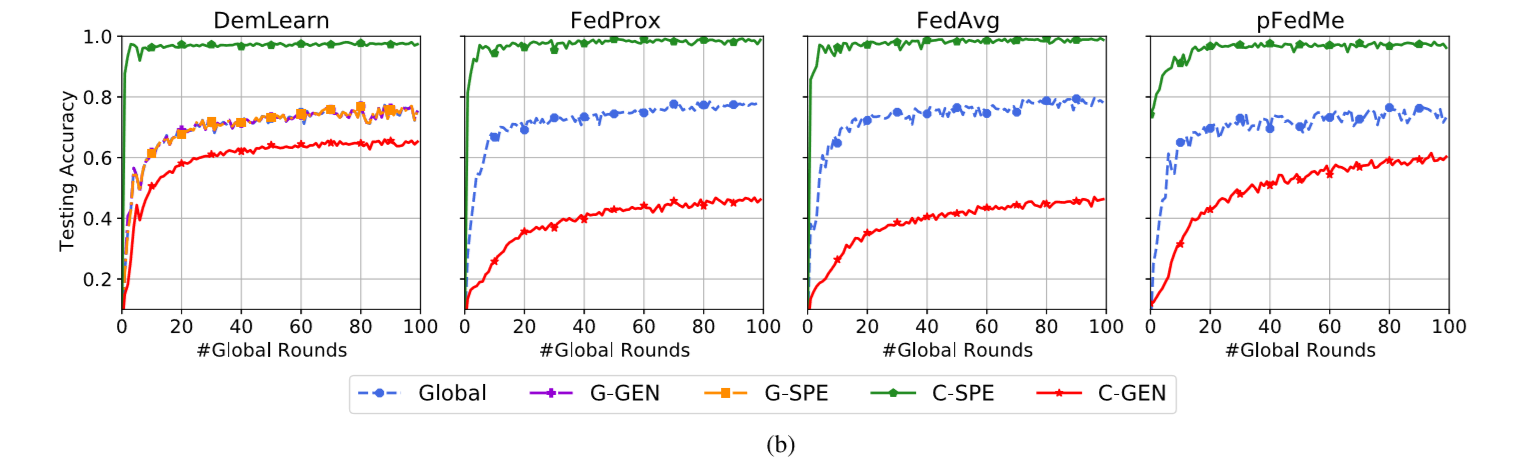
\includegraphics[scale=0.4]{DemLearnFashionMNIST}\\
Anche qui DemLearn è più veloce dei suoi concorrenti con il set dati FashionMNIST\\\\
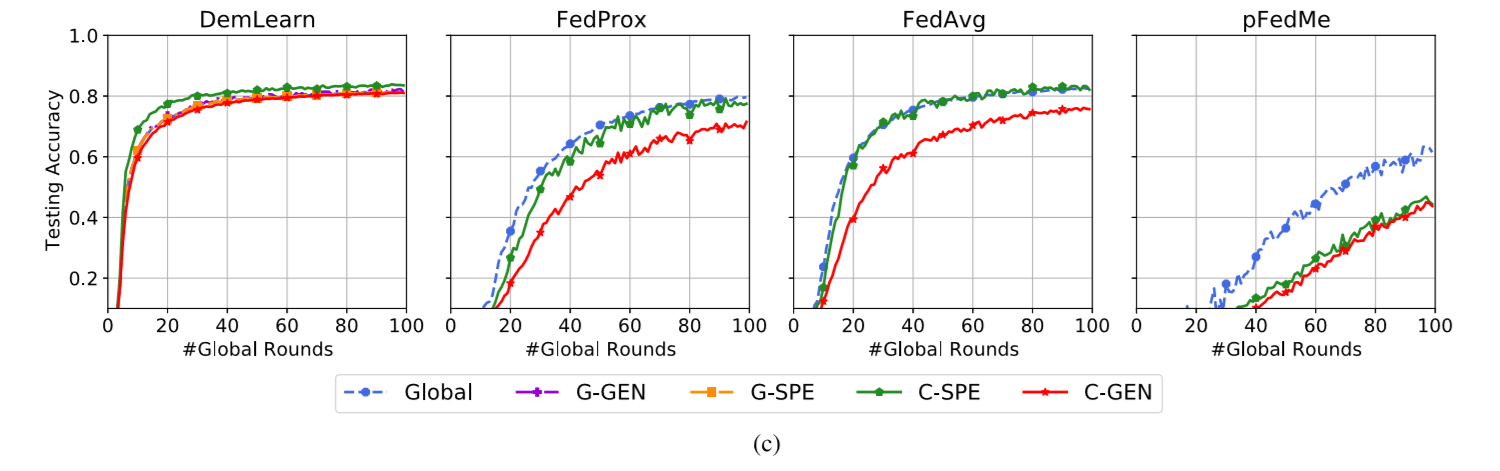
\includegraphics[scale=0.4]{DemLearnFederatedExtMNIST}\\\\
Tutti gli altri algoritmi hanno mostrato prestazioni inferiori e più fluttuanti rispetto a quelle degli altri algoritmi per il set di dati FE-MNIST. pFedMe ottiene un lento miglioramento dei modelli client sia nella specializzazione che nella generalizzazione. Nel frattempo, DemLearn mostra velocità ed efficienza di convergenza stabili per ottenere prestazioni costantemente elevate dei modelli di apprendimento a tutti i livelli.\\\\
\includegraphics[scale=0.5]{cifar10Comparison}\\\\
Osserviamo che DemLearn subisce un leggero degrado delle prestazioni C-SPE e Global per ottenere prestazioni C-GEN elevate. Dopo 100 round, DemLearn dimostra buone capacità di apprendimento di compromesso dei modelli client con C-SPE elevato (79,09\%) prestazioni C-GEN (57\%) e mentre altri algoritmi di base producono solo modelli locali distorti con capacità generalizzate basse.\\\\
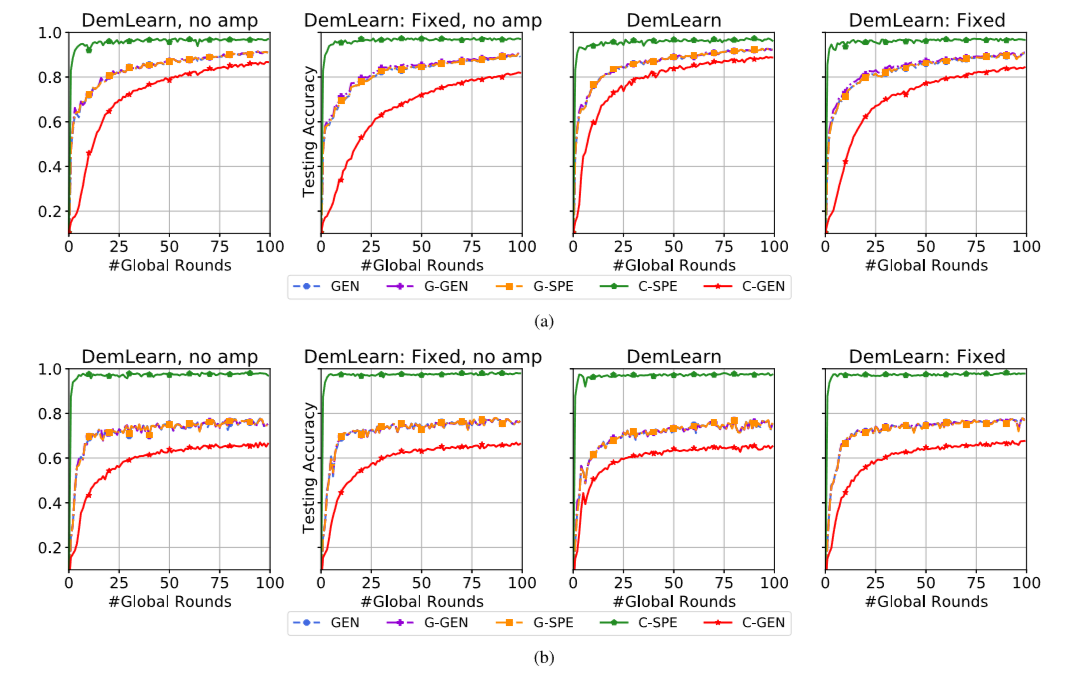
\includegraphics[scale=0.5]{AlgoStructureComp}
Valutiamo e confrontiamo le prestazioni dell'algoritmo proposto per una struttura gerarchica fissa e auto-organizzante attraverso la ricostruzione periodica (cioè, $\tau=1$). Osserviamo che DemLearn beneficia del meccanismo di autoorganizzazione e può fornire una capacità di generalizzazione leggermente migliore dei modelli client. Inoltre, l'amplificazione nei primi cinque cicli aiuta l'algoritmo proposto a velocizzare le prestazioni iniziali dell'algoritmo DemLearn.\\
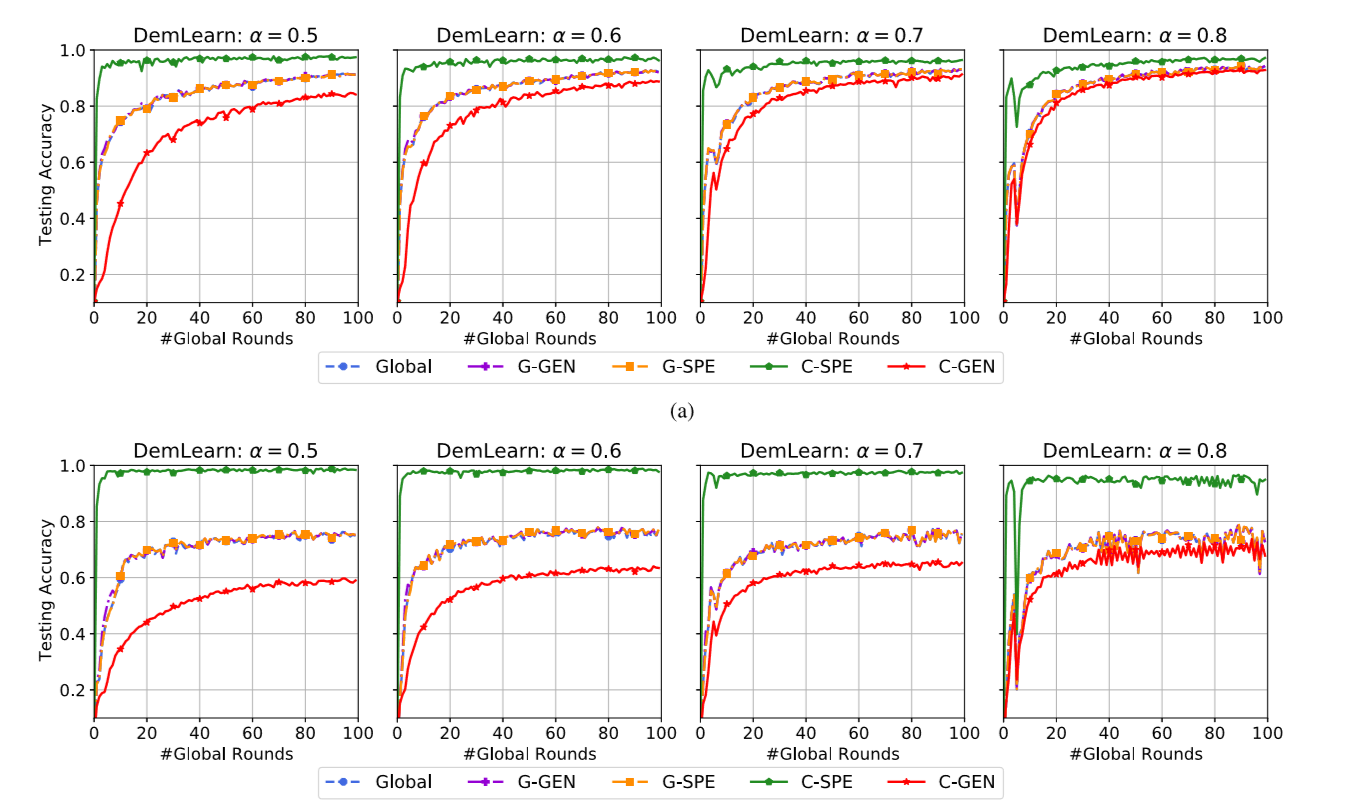
\includegraphics[scale=0.4]{DemAlpha}\\
Mostriamo adesso l'impatto del parametro $\alpha$ nell'accuratezza del test dei set di dati MNIST e Fashion-MNIST, come mostrato. Come si può vedere nei risultati, quando $\alpha$ è grande, otteniamo prestazioni elevate del cliente generalizzazione mentre un leggero degrado nelle loro capacità specializzate.
Pertanto, l'aumento del valore di $\alpha$ migliora la generalizzazione, ma riduce anche in misura marginale le prestazioni di specializzazione dei modelli client. Poiché $\alpha=\mu_{k+1}/(\mu_k+\mu_{k+1})$ controlla il contributo dei modelli di apprendimento del gruppo superiore e dei membri del gruppo, la modifica di $\alpha$ produce l'impatto sulla diffusione della conoscenza generalizzata dai gruppi superiori ai gruppi e ai clienti di livello inferiore. Ad ogni livello k, il valore più alto di $\alpha$ indica che l'obiettivo è più focalizzato sulla minimizzazione del divario con il modello del gruppo superiore a k + 1 rispetto ai modelli del gruppo inferiore a k - 1. Inoltre, valutiamo l'impatto di altri parametri , come $\mu$, K, $\tau$ ma non mostrano effetti evidenti sulle prestazioni di DemLearn probabilmente a causa delle impostazioni di simulazione su piccola scala. Oltre a ciò, ridurre la frequenza degli aggiornamenti del cluster aumentando il parametro $\tau$ può aiutare l'algoritmo a ottenere prestazioni comparabili con un minor costo di riorganizzazione della struttura gerarchica. Tuttavia, a causa della portata limitata dei set di dati e delle impostazioni simulati, si crede che l'impatto dei parametri definiti sulle prestazioni dell'algoritmo proposto si realizzi meglio quando si valuta l'algoritmo con dati più pratici e sperimentali.\\
Oltre alla distanza euclidea tra i parametri di apprendimento nell'algoritmo di clustering gerarchico, possiamo anche valutare la distanza $\phi_{n,t}^{(cos)}$ tra due modelli di apprendimento tramite la somiglianza del coseno con segue:\\
\\ $\phi_{n,t}^{(cos)}=cos(w_n,w_l)=\frac{\sum_{m=1}^M w_{n,m}w_{l,m}}{\sqrt{\sum_{m=1}^M}w_{n,m}^2\sqrt{\sum_{m=1}^M}w_{l,m}^2}$ \hspace{1cm} (11)\\
I risultati sperimentali dimostrano che i modelli client e di gruppo mostrano prestazioni di apprendimento quasi simili e diverse tendenze della topologia del cluster utilizzando l'algoritmo DemLearn. Come mostrato nel Client-GEN, alcuni valori anomali contribuiscono al calo delle prestazioni client-GEN durante la formazione. Allo stesso tempo, la maggior parte dei clienti ha capacità generalizzate paragonabili al modello globale. Di conseguenza, l'illustrazione ci aiuta ulteriormente a capire i clienti estremamente diversi con prestazioni C-GEN basse. Ciò significa che, in ogni round, i valori anomali vengono rilevati (e classificati) da un meccanismo di raggruppamento che è estremamente diverso da altri parametri del modello client. Tuttavia, notiamo che i valori anomali non sono sempre gli stessi e cambiano durante gli aggiornamenti del modello locale. Ma alcuni appaiono più volte e forniscono informazioni significative per il sistema di apprendimento. Inoltre la differenza nella topologia del cluster non influisce molto sulle prestazioni di apprendimento complessive.\\
Rispetto a FedAvg e FedProx, abbiamo un costo computazionale sul dispositivo simile per risolvere il problema PLP utilizzando il metodo di discesa del gradiente. Diversamente dagli altri, pFedMe richiede passaggi aggiuntivi per l'approssimazione $\theta$ e quindi richiede più tempo di calcolo sul dispositivo client. D'altra parte, per il tempo di calcolo richiesto sul server, l'algoritmo DemLearn richiede un costo di calcolo aggiuntivo per il clustering gerarchico e un costo trascurabile per gli aggiornamenti gerarchici. Notiamo che il costo del clustering gerarchico dipende dalla dimensione del modello e dal numero di agenti di apprendimento. In linea di principio, l'algoritmo standard per il clustering gerarchico agglomerativo ha una complessità temporale di O(n3) e richiede una memoria O(n2) [24].Valutiamo l'algoritmo con n = 50 utenti e otteniamo in media un tempo di esecuzione di 0,0015 secondi per passo quando si utilizza un computer con CPU i7-7700K e una memoria di 32 GB. Per il costo di comunicazione, tutti gli algoritmi richiedono costi simili per inviare i parametri del modello.\\\\
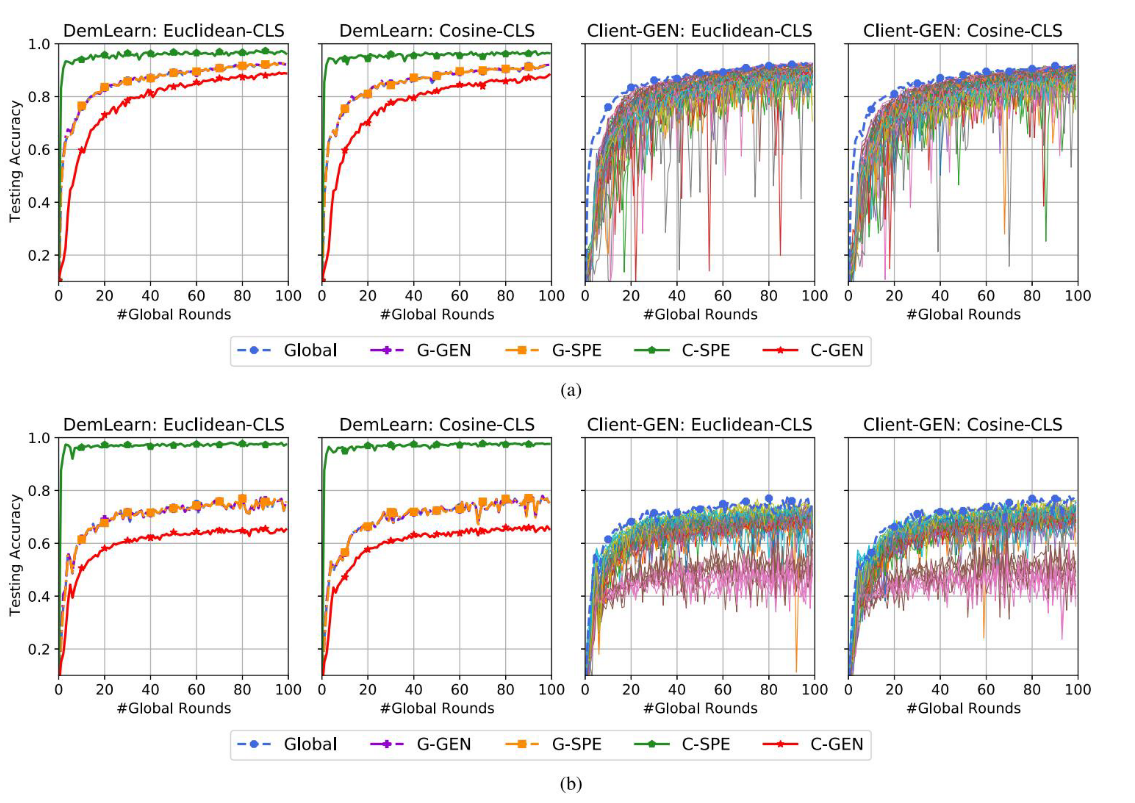
\includegraphics[scale=0.4]{ClusteringLast}\\\\
In pratica, per implementare una tipica struttura gerarchica, i sistemi Dem-AI possono includere tre entità. Un server cloud che gestisce il modello globale (nodo radice) e i suoi gruppi generalizzati di sottolivello. Server regionali distribuiti, che sono server perimetrali distribuiti all'interno di ciascuna regione e il cui ruolo è gestire i sottogruppi e gli agenti di apprendimento e agenti di apprendimento.
Purtroppo l'implementazione per il clustering gerarchico è centralizzata in questi esperimenti. Tuttavia, il meccanismo di clustering gerarchico agglomerante unisce gli agenti e i gruppi di apprendimento dal basso verso l'alto, e quindi è possibile implementarlo in modo decentralizzato. Pertanto, possiamo gestire il clustering gerarchico nel server cloud per i livelli superiori e l'implementazione decentralizzata per le regioni nei server perimetrali per i gruppi di livello inferiore. Inoltre, questo meccanismo di raggruppamento può mitigare gli effetti negativi dell'aggregazione di agenti di apprendimento estremamente diversi per costruire modelli gerarchici generalizzati. In questo modo, manteniamo tre o più livelli di modelli generalizzati invece di un unico modello globale. Per quanto ne sappiamo, questo design non è stato ancora preso in considerazione in recenti studi sul FL personalizzato.